\documentclass{standalone}
\usepackage{tikz}
\usetikzlibrary{patterns, positioning}

\begin{document}
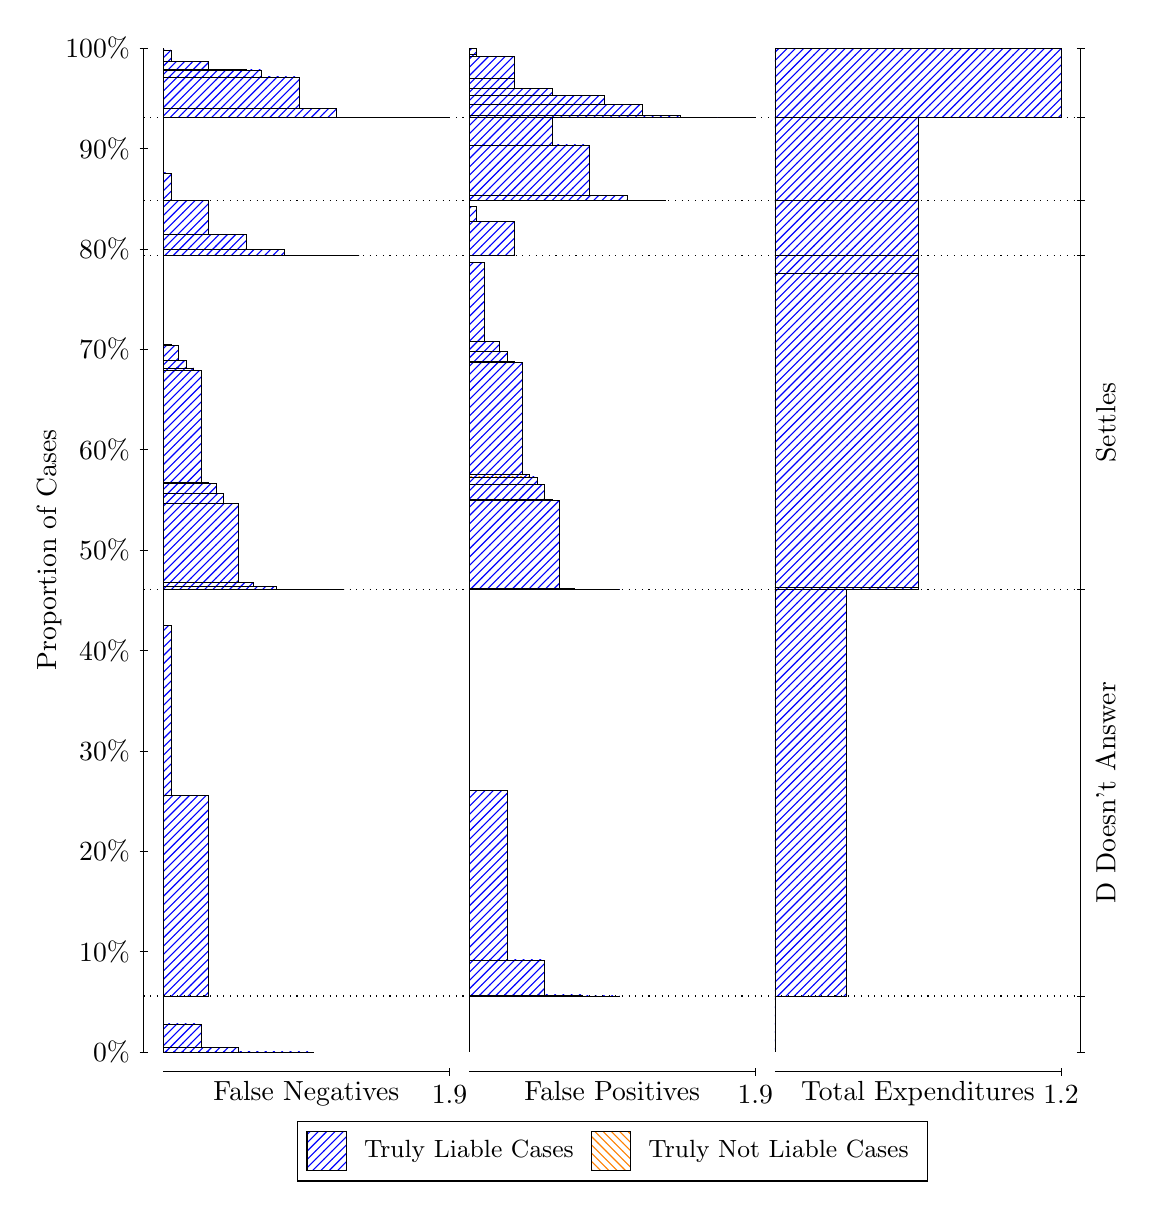
\begin{tikzpicture}
\draw[black, very thin] (1.5,1.75) -- (1.5,14.5);
\node[rotate=90, anchor=center] at (0.3, 8.125) {Proportion of Cases};
\draw[black, very thin] (1.45,1.75) -- (1.55,1.75);
\node[anchor=east] at (1.45, 1.75) {0\%};
\draw[black, very thin] (1.45,3.025) -- (1.55,3.025);
\node[anchor=east] at (1.45, 3.025) {10\%};
\draw[black, very thin] (1.45,4.3) -- (1.55,4.3);
\node[anchor=east] at (1.45, 4.3) {20\%};
\draw[black, very thin] (1.45,5.575) -- (1.55,5.575);
\node[anchor=east] at (1.45, 5.575) {30\%};
\draw[black, very thin] (1.45,6.85) -- (1.55,6.85);
\node[anchor=east] at (1.45, 6.85) {40\%};
\draw[black, very thin] (1.45,8.125) -- (1.55,8.125);
\node[anchor=east] at (1.45, 8.125) {50\%};
\draw[black, very thin] (1.45,9.4) -- (1.55,9.4);
\node[anchor=east] at (1.45, 9.4) {60\%};
\draw[black, very thin] (1.45,10.675) -- (1.55,10.675);
\node[anchor=east] at (1.45, 10.675) {70\%};
\draw[black, very thin] (1.45,11.95) -- (1.55,11.95);
\node[anchor=east] at (1.45, 11.95) {80\%};
\draw[black, very thin] (1.45,13.225) -- (1.55,13.225);
\node[anchor=east] at (1.45, 13.225) {90\%};
\draw[black, very thin] (1.45,14.5) -- (1.55,14.5);
\node[anchor=east] at (1.45, 14.5) {100\%};

\draw[black, very thin] (13.4,1.75) -- (13.4,14.5);
\draw[black, very thin] (13.35,1.75) -- (13.45,1.75);
\node[anchor=west] at (13.35, 1.75) {};
\draw[black, very thin] (13.35,2.4609) -- (13.45,2.4609);
\node[anchor=west] at (13.35, 2.4609) {};
\draw[black, very thin] (13.35,7.6219) -- (13.45,7.6219);
\node[anchor=west] at (13.35, 7.6219) {};
\draw[black, very thin] (13.35,11.869) -- (13.45,11.869);
\node[anchor=west] at (13.35, 11.869) {};
\draw[black, very thin] (13.35,12.565) -- (13.45,12.565);
\node[anchor=west] at (13.35, 12.565) {};
\draw[black, very thin] (13.35,13.619) -- (13.45,13.619);
\node[anchor=west] at (13.35, 13.619) {};
\draw[black, very thin] (13.35,14.5) -- (13.45,14.5);
\node[anchor=west] at (13.35, 14.5) {};

\draw[black, very thin, pattern color=blue, pattern=north east lines] (1.75,1.75) rectangle (3.6623,1.75);
\draw[black, very thin, pattern color=blue, pattern=north east lines] (1.75,1.75) rectangle (3.1842,1.7505);
\draw[black, very thin, pattern color=blue, pattern=north east lines] (1.75,1.7505) rectangle (2.7061,1.8069);
\draw[black, very thin, pattern color=blue, pattern=north east lines] (1.75,1.8069) rectangle (2.2281,2.106);
\draw[black, very thin, pattern color=orange, pattern=north west lines] (1.75,2.106) rectangle (1.75,2.106);
\draw[black, very thin, pattern color=blue, pattern=north east lines] (1.75,2.106) rectangle (1.75,2.4609);
\draw[black, very thin, pattern color=blue, pattern=north east lines] (1.75,2.4609) rectangle (2.3237,5.0069);
\draw[black, very thin, pattern color=blue, pattern=north east lines] (1.75,5.0069) rectangle (1.8456,7.1631);
\draw[black, very thin, pattern color=orange, pattern=north west lines] (1.75,7.1631) rectangle (1.75,7.1631);
\draw[black, very thin, pattern color=blue, pattern=north east lines] (1.75,7.1631) rectangle (1.75,7.6219);
\draw[black, very thin, pattern color=blue, pattern=north east lines] (1.75,7.6219) rectangle (4.0447,7.6219);
\draw[black, very thin, pattern color=blue, pattern=north east lines] (1.75,7.6219) rectangle (3.8535,7.6219);
\draw[black, very thin, pattern color=blue, pattern=north east lines] (1.75,7.6219) rectangle (3.6623,7.6219);
\draw[black, very thin, pattern color=blue, pattern=north east lines] (1.75,7.6219) rectangle (3.5667,7.6219);
\draw[black, very thin, pattern color=blue, pattern=north east lines] (1.75,7.6219) rectangle (3.4711,7.6219);
\draw[black, very thin, pattern color=blue, pattern=north east lines] (1.75,7.6219) rectangle (3.4711,7.6219);
\draw[black, very thin, pattern color=blue, pattern=north east lines] (1.75,7.6219) rectangle (3.3754,7.6232);
\draw[black, very thin, pattern color=blue, pattern=north east lines] (1.75,7.6232) rectangle (3.2798,7.6232);
\draw[black, very thin, pattern color=blue, pattern=north east lines] (1.75,7.6232) rectangle (3.1842,7.6584);
\draw[black, very thin, pattern color=blue, pattern=north east lines] (1.75,7.6584) rectangle (3.0886,7.6586);
\draw[black, very thin, pattern color=blue, pattern=north east lines] (1.75,7.6586) rectangle (2.993,7.6586);
\draw[black, very thin, pattern color=blue, pattern=north east lines] (1.75,7.6586) rectangle (2.993,7.6634);
\draw[black, very thin, pattern color=blue, pattern=north east lines] (1.75,7.6634) rectangle (2.8974,7.6634);
\draw[black, very thin, pattern color=blue, pattern=north east lines] (1.75,7.6634) rectangle (2.8974,7.709);
\draw[black, very thin, pattern color=blue, pattern=north east lines] (1.75,7.709) rectangle (2.8018,7.7097);
\draw[black, very thin, pattern color=blue, pattern=north east lines] (1.75,7.7097) rectangle (2.7061,8.7136);
\draw[black, very thin, pattern color=blue, pattern=north east lines] (1.75,8.7136) rectangle (2.6105,8.7136);
\draw[black, very thin, pattern color=blue, pattern=north east lines] (1.75,8.7136) rectangle (2.6105,8.7191);
\draw[black, very thin, pattern color=blue, pattern=north east lines] (1.75,8.7191) rectangle (2.5149,8.7191);
\draw[black, very thin, pattern color=blue, pattern=north east lines] (1.75,8.7191) rectangle (2.5149,8.841);
\draw[black, very thin, pattern color=blue, pattern=north east lines] (1.75,8.841) rectangle (2.4193,8.841);
\draw[black, very thin, pattern color=blue, pattern=north east lines] (1.75,8.841) rectangle (2.4193,8.9697);
\draw[black, very thin, pattern color=blue, pattern=north east lines] (1.75,8.9697) rectangle (2.3237,8.9871);
\draw[black, very thin, pattern color=blue, pattern=north east lines] (1.75,8.9871) rectangle (2.2281,10.408);
\draw[black, very thin, pattern color=blue, pattern=north east lines] (1.75,10.408) rectangle (2.1325,10.408);
\draw[black, very thin, pattern color=blue, pattern=north east lines] (1.75,10.408) rectangle (2.1325,10.437);
\draw[black, very thin, pattern color=blue, pattern=north east lines] (1.75,10.437) rectangle (2.0368,10.437);
\draw[black, very thin, pattern color=blue, pattern=north east lines] (1.75,10.437) rectangle (2.0368,10.53);
\draw[black, very thin, pattern color=blue, pattern=north east lines] (1.75,10.53) rectangle (1.9412,10.53);
\draw[black, very thin, pattern color=blue, pattern=north east lines] (1.75,10.53) rectangle (1.9412,10.726);
\draw[black, very thin, pattern color=blue, pattern=north east lines] (1.75,10.726) rectangle (1.8456,10.736);
\draw[black, very thin, pattern color=orange, pattern=north west lines] (1.75,10.736) rectangle (1.75,10.736);
\draw[black, very thin, pattern color=blue, pattern=north east lines] (1.75,10.736) rectangle (1.75,11.869);
\draw[black, very thin, pattern color=blue, pattern=north east lines] (1.75,11.869) rectangle (4.236,11.869);
\draw[black, very thin, pattern color=blue, pattern=north east lines] (1.75,11.869) rectangle (3.7579,11.871);
\draw[black, very thin, pattern color=blue, pattern=north east lines] (1.75,11.871) rectangle (3.2798,11.942);
\draw[black, very thin, pattern color=blue, pattern=north east lines] (1.75,11.942) rectangle (2.8018,12.138);
\draw[black, very thin, pattern color=blue, pattern=north east lines] (1.75,12.138) rectangle (2.3237,12.565);
\draw[black, very thin, pattern color=orange, pattern=north west lines] (1.75,12.565) rectangle (1.75,12.565);
\draw[black, very thin, pattern color=blue, pattern=north east lines] (1.75,12.565) rectangle (2.3237,12.569);
\draw[black, very thin, pattern color=blue, pattern=north east lines] (1.75,12.569) rectangle (1.8456,12.915);
\draw[black, very thin, pattern color=orange, pattern=north west lines] (1.75,12.915) rectangle (1.75,12.915);
\draw[black, very thin, pattern color=blue, pattern=north east lines] (1.75,12.915) rectangle (1.75,13.619);
\draw[black, very thin, pattern color=blue, pattern=north east lines] (1.75,13.619) rectangle (5.3833,13.619);
\draw[black, very thin, pattern color=blue, pattern=north east lines] (1.75,13.619) rectangle (4.9053,13.619);
\draw[black, very thin, pattern color=blue, pattern=north east lines] (1.75,13.619) rectangle (4.4272,13.622);
\draw[black, very thin, pattern color=blue, pattern=north east lines] (1.75,13.622) rectangle (3.9491,13.73);
\draw[black, very thin, pattern color=blue, pattern=north east lines] (1.75,13.73) rectangle (3.7579,13.73);
\draw[black, very thin, pattern color=blue, pattern=north east lines] (1.75,13.73) rectangle (3.4711,14.134);
\draw[black, very thin, pattern color=blue, pattern=north east lines] (1.75,14.134) rectangle (3.2798,14.134);
\draw[black, very thin, pattern color=blue, pattern=north east lines] (1.75,14.134) rectangle (2.993,14.223);
\draw[black, very thin, pattern color=blue, pattern=north east lines] (1.75,14.223) rectangle (2.8018,14.225);
\draw[black, very thin, pattern color=blue, pattern=north east lines] (1.75,14.225) rectangle (2.5149,14.225);
\draw[black, very thin, pattern color=blue, pattern=north east lines] (1.75,14.225) rectangle (2.3237,14.225);
\draw[black, very thin, pattern color=blue, pattern=north east lines] (1.75,14.225) rectangle (2.3237,14.33);
\draw[black, very thin, pattern color=blue, pattern=north east lines] (1.75,14.33) rectangle (1.8456,14.331);
\draw[black, very thin, pattern color=blue, pattern=north east lines] (1.75,14.331) rectangle (1.8456,14.477);
\draw[black, very thin, pattern color=orange, pattern=north west lines] (1.75,14.477) rectangle (1.75,14.477);
\draw[black, very thin, pattern color=blue, pattern=north east lines] (1.75,14.477) rectangle (1.75,14.5);
\draw[black, very thin, pattern color=orange, pattern=north west lines] (5.6333,1.75) rectangle (5.6333,1.75);
\draw[black, very thin, pattern color=blue, pattern=north east lines] (5.6333,1.75) rectangle (5.6333,2.4609);
\draw[black, very thin, pattern color=orange, pattern=north west lines] (5.6333,2.4609) rectangle (7.5456,2.4609);
\draw[black, very thin, pattern color=blue, pattern=north east lines] (5.6333,2.4609) rectangle (7.5456,2.461);
\draw[black, very thin, pattern color=blue, pattern=north east lines] (5.6333,2.461) rectangle (7.0675,2.4744);
\draw[black, very thin, pattern color=blue, pattern=north east lines] (5.6333,2.4744) rectangle (6.5895,2.9197);
\draw[black, very thin, pattern color=blue, pattern=north east lines] (5.6333,2.9197) rectangle (6.1114,5.0759);
\draw[black, very thin, pattern color=blue, pattern=north east lines] (5.6333,5.0759) rectangle (5.6333,7.6219);
\draw[black, very thin, pattern color=orange, pattern=north west lines] (5.6333,7.6219) rectangle (7.5456,7.6219);
\draw[black, very thin, pattern color=blue, pattern=north east lines] (5.6333,7.6219) rectangle (7.5456,7.6219);
\draw[black, very thin, pattern color=orange, pattern=north west lines] (5.6333,7.6219) rectangle (7.3544,7.6219);
\draw[black, very thin, pattern color=blue, pattern=north east lines] (5.6333,7.6219) rectangle (7.3544,7.6219);
\draw[black, very thin, pattern color=orange, pattern=north west lines] (5.6333,7.6219) rectangle (7.1632,7.6219);
\draw[black, very thin, pattern color=blue, pattern=north east lines] (5.6333,7.6219) rectangle (7.1632,7.6244);
\draw[black, very thin, pattern color=blue, pattern=north east lines] (5.6333,7.6244) rectangle (7.0675,7.6244);
\draw[black, very thin, pattern color=orange, pattern=north west lines] (5.6333,7.6244) rectangle (6.9719,7.6244);
\draw[black, very thin, pattern color=blue, pattern=north east lines] (5.6333,7.6244) rectangle (6.9719,7.639);
\draw[black, very thin, pattern color=blue, pattern=north east lines] (5.6333,7.639) rectangle (6.8763,7.639);
\draw[black, very thin, pattern color=orange, pattern=north west lines] (5.6333,7.639) rectangle (6.7807,7.639);
\draw[black, very thin, pattern color=blue, pattern=north east lines] (5.6333,7.639) rectangle (6.7807,8.7549);
\draw[black, very thin, pattern color=blue, pattern=north east lines] (5.6333,8.7549) rectangle (6.6851,8.7649);
\draw[black, very thin, pattern color=orange, pattern=north west lines] (5.6333,8.7649) rectangle (6.5895,8.7649);
\draw[black, very thin, pattern color=blue, pattern=north east lines] (5.6333,8.7649) rectangle (6.5895,8.9604);
\draw[black, very thin, pattern color=blue, pattern=north east lines] (5.6333,8.9604) rectangle (6.4939,9.0532);
\draw[black, very thin, pattern color=orange, pattern=north west lines] (5.6333,9.0532) rectangle (6.3982,9.0532);
\draw[black, very thin, pattern color=blue, pattern=north east lines] (5.6333,9.0532) rectangle (6.3982,9.0824);
\draw[black, very thin, pattern color=blue, pattern=north east lines] (5.6333,9.0824) rectangle (6.3982,9.0824);
\draw[black, very thin, pattern color=blue, pattern=north east lines] (5.6333,9.0824) rectangle (6.3026,10.503);
\draw[black, very thin, pattern color=blue, pattern=north east lines] (5.6333,10.503) rectangle (6.207,10.521);
\draw[black, very thin, pattern color=blue, pattern=north east lines] (5.6333,10.521) rectangle (6.1114,10.65);
\draw[black, very thin, pattern color=blue, pattern=north east lines] (5.6333,10.65) rectangle (6.0158,10.771);
\draw[black, very thin, pattern color=blue, pattern=north east lines] (5.6333,10.771) rectangle (5.9202,10.777);
\draw[black, very thin, pattern color=blue, pattern=north east lines] (5.6333,10.777) rectangle (5.9202,10.777);
\draw[black, very thin, pattern color=blue, pattern=north east lines] (5.6333,10.777) rectangle (5.8246,11.781);
\draw[black, very thin, pattern color=blue, pattern=north east lines] (5.6333,11.781) rectangle (5.7289,11.782);
\draw[black, very thin, pattern color=blue, pattern=north east lines] (5.6333,11.782) rectangle (5.6333,11.869);
\draw[black, very thin, pattern color=orange, pattern=north west lines] (5.6333,11.869) rectangle (6.207,11.869);
\draw[black, very thin, pattern color=blue, pattern=north east lines] (5.6333,11.869) rectangle (6.207,12.296);
\draw[black, very thin, pattern color=blue, pattern=north east lines] (5.6333,12.296) rectangle (5.7289,12.491);
\draw[black, very thin, pattern color=blue, pattern=north east lines] (5.6333,12.491) rectangle (5.6333,12.565);
\draw[black, very thin, pattern color=orange, pattern=north west lines] (5.6333,12.565) rectangle (8.1193,12.565);
\draw[black, very thin, pattern color=blue, pattern=north east lines] (5.6333,12.565) rectangle (8.1193,12.566);
\draw[black, very thin, pattern color=blue, pattern=north east lines] (5.6333,12.566) rectangle (7.6412,12.628);
\draw[black, very thin, pattern color=blue, pattern=north east lines] (5.6333,12.628) rectangle (7.1632,13.269);
\draw[black, very thin, pattern color=blue, pattern=north east lines] (5.6333,13.269) rectangle (6.6851,13.615);
\draw[black, very thin, pattern color=blue, pattern=north east lines] (5.6333,13.615) rectangle (6.207,13.619);
\draw[black, very thin, pattern color=orange, pattern=north west lines] (5.6333,13.619) rectangle (9.2667,13.619);
\draw[black, very thin, pattern color=blue, pattern=north east lines] (5.6333,13.619) rectangle (9.2667,13.619);
\draw[black, very thin, pattern color=orange, pattern=north west lines] (5.6333,13.619) rectangle (8.7886,13.619);
\draw[black, very thin, pattern color=blue, pattern=north east lines] (5.6333,13.619) rectangle (8.7886,13.619);
\draw[black, very thin, pattern color=orange, pattern=north west lines] (5.6333,13.619) rectangle (8.3105,13.619);
\draw[black, very thin, pattern color=blue, pattern=north east lines] (5.6333,13.619) rectangle (8.3105,13.642);
\draw[black, very thin, pattern color=orange, pattern=north west lines] (5.6333,13.642) rectangle (7.8325,13.642);
\draw[black, very thin, pattern color=blue, pattern=north east lines] (5.6333,13.642) rectangle (7.8325,13.789);
\draw[black, very thin, pattern color=blue, pattern=north east lines] (5.6333,13.789) rectangle (7.3544,13.894);
\draw[black, very thin, pattern color=orange, pattern=north west lines] (5.6333,13.894) rectangle (7.1632,13.894);
\draw[black, very thin, pattern color=blue, pattern=north east lines] (5.6333,13.894) rectangle (7.1632,13.894);
\draw[black, very thin, pattern color=blue, pattern=north east lines] (5.6333,13.894) rectangle (6.8763,13.896);
\draw[black, very thin, pattern color=orange, pattern=north west lines] (5.6333,13.896) rectangle (6.6851,13.896);
\draw[black, very thin, pattern color=blue, pattern=north east lines] (5.6333,13.896) rectangle (6.6851,13.985);
\draw[black, very thin, pattern color=blue, pattern=north east lines] (5.6333,13.985) rectangle (6.3982,13.985);
\draw[black, very thin, pattern color=blue, pattern=north east lines] (5.6333,13.985) rectangle (6.207,14.118);
\draw[black, very thin, pattern color=orange, pattern=north west lines] (5.6333,14.118) rectangle (6.207,14.118);
\draw[black, very thin, pattern color=blue, pattern=north east lines] (5.6333,14.118) rectangle (6.207,14.389);
\draw[black, very thin, pattern color=blue, pattern=north east lines] (5.6333,14.389) rectangle (5.9202,14.389);
\draw[black, very thin, pattern color=blue, pattern=north east lines] (5.6333,14.389) rectangle (5.7289,14.421);
\draw[black, very thin, pattern color=blue, pattern=north east lines] (5.6333,14.421) rectangle (5.7289,14.497);
\draw[black, very thin, pattern color=blue, pattern=north east lines] (5.6333,14.497) rectangle (5.6333,14.5);
\draw[black, very thin, pattern color=orange, pattern=north west lines] (9.5167,1.75) rectangle (9.5167,1.75);
\draw[black, very thin, pattern color=blue, pattern=north east lines] (9.5167,1.75) rectangle (9.5167,2.4609);
\draw[black, very thin, pattern color=orange, pattern=north west lines] (9.5167,2.4609) rectangle (10.425,2.4609);
\draw[black, very thin, pattern color=blue, pattern=north east lines] (9.5167,2.4609) rectangle (10.425,7.6219);
\draw[black, very thin, pattern color=orange, pattern=north west lines] (9.5167,7.6219) rectangle (11.333,7.6219);
\draw[black, very thin, pattern color=blue, pattern=north east lines] (9.5167,7.6219) rectangle (11.333,7.6526);
\draw[black, very thin, pattern color=orange, pattern=north west lines] (9.5167,7.6526) rectangle (11.333,7.6526);
\draw[black, very thin, pattern color=blue, pattern=north east lines] (9.5167,7.6526) rectangle (11.333,11.635);
\draw[black, very thin, pattern color=orange, pattern=north west lines] (9.5167,11.635) rectangle (11.333,11.635);
\draw[black, very thin, pattern color=blue, pattern=north east lines] (9.5167,11.635) rectangle (11.333,11.869);
\draw[black, very thin, pattern color=orange, pattern=north west lines] (9.5167,11.869) rectangle (11.333,11.869);
\draw[black, very thin, pattern color=blue, pattern=north east lines] (9.5167,11.869) rectangle (11.333,12.565);
\draw[black, very thin, pattern color=orange, pattern=north west lines] (9.5167,12.565) rectangle (11.333,12.565);
\draw[black, very thin, pattern color=blue, pattern=north east lines] (9.5167,12.565) rectangle (11.333,13.619);
\draw[black, very thin, pattern color=orange, pattern=north west lines] (9.5167,13.619) rectangle (13.15,13.619);
\draw[black, very thin, pattern color=blue, pattern=north east lines] (9.5167,13.619) rectangle (13.15,14.5);
\draw[black, dotted] (1.5,2.4609) -- (13.4,2.4609);
\draw[black, dotted] (1.5,7.6219) -- (13.4,7.6219);
\draw[black, dotted] (1.5,11.869) -- (13.4,11.869);
\draw[black, dotted] (1.5,12.565) -- (13.4,12.565);
\draw[black, dotted] (1.5,13.619) -- (13.4,13.619);
\draw[black, very thin] (1.75,1.5) -- (5.3833,1.5);
\node[anchor=north] at (3.5667, 1.5) {False Negatives};
\draw[black, very thin] (5.3833,1.45) -- (5.3833,1.55);
\node[anchor=north] at (5.3833, 1.45) {1.9};

\draw[black, very thin] (5.6333,1.5) -- (9.2667,1.5);
\node[anchor=north] at (7.45, 1.5) {False Positives};
\draw[black, very thin] (9.2667,1.45) -- (9.2667,1.55);
\node[anchor=north] at (9.2667, 1.45) {1.9};

\draw[black, very thin] (9.5167,1.5) -- (13.15,1.5);
\node[anchor=north] at (11.333, 1.5) {Total Expenditures};
\draw[black, very thin] (13.15,1.45) -- (13.15,1.55);
\node[anchor=north] at (13.15, 1.45) {1.2};


\node[black, centered, rotate=90] at (13.72, 5.0414) {D Doesn't Answer};
\node[black, centered, rotate=90] at (13.72, 9.7453) {Settles};




\draw (7.449999999999999,1.5) node[draw=none] (baseCoordinate) {};
\begin{scope}[align=center]
        \matrix[scale=0.5, draw=black, below=0.5cm of baseCoordinate, nodes={draw}, column sep=0.1cm]{
            \node[rectangle, draw, minimum width=0.5cm, minimum height=0.5cm, pattern=north east lines, pattern color=blue] {}; &
            \node[draw=none, font=\small] (B) {Truly Liable Cases}; &
            \node[rectangle, draw, minimum width=0.5cm, minimum height=0.5cm, pattern=north west lines, pattern color=orange] {}; &
            \node[draw=none, font=\small] (B) {Truly Not Liable Cases}; \\
            };
\end{scope}

\end{tikzpicture}
\end{document}